%\begin{figure*}[t]
%	\addtolength{\tabcolsep}{-4.5pt}
%	\begin{tabular}{ccccccccc}
%		& \multicolumn{2}{c}{\toptext{2\resultwidth}{Point estimate}} & \multicolumn{5}{c}{\toptext{5\resultwidth}{Bayesian inference}}\\[-4pt]
%		target & loss & optimize & posterior & sample-1 & sample-2 & sample-3& sample-4
%		\\
%		
\includegraphics[width=\resultwidth]{synth/bump/target.jpg} &
%		\includegraphics[width=\resultwidth]{synth/bump/loss.pdf} &
%		\includegraphics[width=\resultwidth]{synth/bump/optim.jpg} &
%		\includegraphics[width=\resultwidth]{synth/bump/posterior.pdf} &
%		\includegraphics[width=\resultwidth]{synth/bump/good1.jpg} &
%		\includegraphics[width=\resultwidth]{synth/bump/good2.jpg} &
%		\includegraphics[width=\resultwidth]{synth/bump/good3.jpg} &
%		\includegraphics[width=\resultwidth]{synth/bump/bad1.jpg}
%		\\
%		
\includegraphics[width=\resultwidth]{synth/leather/target.jpg} &
%		\includegraphics[width=\resultwidth]{synth/leather/loss.pdf} &
%		\includegraphics[width=\resultwidth]{synth/leather/optim.jpg} &
%		\includegraphics[width=\resultwidth]{synth/leather/posterior.pdf} &
%		\includegraphics[width=\resultwidth]{synth/leather/good1.jpg} &
%		\includegraphics[width=\resultwidth]{synth/leather/good2.jpg} &
%		\includegraphics[width=\resultwidth]{synth/leather/good3.jpg} &
%		\includegraphics[width=\resultwidth]{synth/leather/bad1.jpg}
%		\\
%		
\includegraphics[width=\resultwidth]{synth/plaster/target.jpg} &
%		\includegraphics[width=\resultwidth]{synth/plaster/loss.pdf} &
%		\includegraphics[width=\resultwidth]{synth/plaster/optim.jpg} &
%		\includegraphics[width=\resultwidth]{synth/plaster/posterior.pdf} &
%		\includegraphics[width=\resultwidth]{synth/plaster/good1.jpg} &
%		\includegraphics[width=\resultwidth]{synth/plaster/good2.jpg} &
%		\includegraphics[width=\resultwidth]{synth/plaster/good3.jpg} &
%		\includegraphics[width=\resultwidth]{synth/plaster/bad1.jpg}
%		\\
%		
\includegraphics[width=\resultwidth]{synth/flake/target.jpg} &
%		\includegraphics[width=\resultwidth]{synth/flake/loss.pdf} &
%		\includegraphics[width=\resultwidth]{synth/flake/optim.jpg} &
%		\includegraphics[width=\resultwidth]{synth/flake/posterior.pdf} &
%		\includegraphics[width=\resultwidth]{synth/flake/good1.jpg} &
%		\includegraphics[width=\resultwidth]{synth/flake/good2.jpg} &
%		\includegraphics[width=\resultwidth]{synth/flake/good3.jpg} &
%		\includegraphics[width=\resultwidth]{synth/flake/bad1.jpg}
%		\\
%		
\includegraphics[width=\resultwidth]{synth/metal/target.jpg} &
%		\includegraphics[width=\resultwidth]{synth/metal/loss.pdf} &
%		\includegraphics[width=\resultwidth]{synth/metal/optim.jpg} &
%		\includegraphics[width=\resultwidth]{synth/metal/posterior.pdf} &
%		\includegraphics[width=\resultwidth]{synth/metal/good1.jpg} &
%		\includegraphics[width=\resultwidth]{synth/metal/good2.jpg} &
%		\includegraphics[width=\resultwidth]{synth/metal/good3.jpg} &
%		\includegraphics[width=\resultwidth]{synth/metal/bad1.jpg}
%		\\
%		
\includegraphics[width=\resultwidth]{synth/wood/target.jpg} &
%		\includegraphics[width=\resultwidth]{synth/wood/loss.pdf} &
%		\includegraphics[width=\resultwidth]{synth/wood/optim.jpg} &
%		\includegraphics[width=\resultwidth]{synth/wood/posterior.pdf} &
%		\includegraphics[width=\resultwidth]{synth/wood/good1.jpg} &
%		\includegraphics[width=\resultwidth]{synth/wood/good2.jpg} &
%		\includegraphics[width=\resultwidth]{synth/wood/good3.jpg} &
%		\includegraphics[width=\resultwidth]{synth/wood/bad1.jpg}
%		\\
%		& & \qquad \qquad \, low &
%		\includegraphics[width=\resultwidthpdf]{img/colorbar.jpg} &
%		high \qquad \qquad \,& & &
%	\end{tabular}
%	%
%	\caption{\label{fig:synth}
%		\textbf{Optimization and HMC sampling on synthetic images.} Each row corresponds to a different material. From top: bump, leather, plaster, metallic flake, brushed metal and wood. Column 1 is rendered images using different forward models. We show optimization results in columns 2 and 3, samplings in the rest columns. For high dimensional posterior visualization, we project them to 2D using PCA. Here we only show the first two major components. The three red dots corresponding to sample-1,2,3, which are closer to the peak of high dimensional distribution. and the green dot (sample-4) is the opposite. More results please refer to supplemental materials.
%	}
%\end{figure*}

\begin{figure*}[t]
	\centering
	\addtolength{\tabcolsep}{-4.5pt}
	\begin{tabular}{ccccccccc}
		target & sample-1 & sample-2 & sample-3 & & target & sample-1 & sample-2 & sample-3
		\\
		\begin{overpic}[width=\resultwidth]{synth/bump_1/target.jpg}
			\imglabel{Bump-1}
		\end{overpic} &
		\includegraphics[width=\resultwidth]{synth/bump_1/good1.jpg} &
		\includegraphics[width=\resultwidth]{synth/bump_1/good2.jpg} &
		\includegraphics[width=\resultwidth]{synth/bump_1/bad1.jpg} &
		&
		\begin{overpic}[width=\resultwidth]{synth/bump_2/target.jpg}
			\imglabel{Bump-2}
		\end{overpic} &
		\includegraphics[width=\resultwidth]{synth/bump_2/good1.jpg} &
		\includegraphics[width=\resultwidth]{synth/bump_2/good2.jpg} &
		\includegraphics[width=\resultwidth]{synth/bump_2/bad1.jpg}
		\\
		\begin{overpic}[width=\resultwidth]{synth/leather_1/target.jpg}
			\imglabel{Leather-1}
		\end{overpic} &
		\includegraphics[width=\resultwidth]{synth/leather_1/good1.jpg} &
		\includegraphics[width=\resultwidth]{synth/leather_1/good2.jpg} &
		\includegraphics[width=\resultwidth]{synth/leather_1/bad1.jpg} &
		&
		\begin{overpic}[width=\resultwidth]{synth/leather_2/target.jpg}
			\imglabel{Leather-2}
		\end{overpic} &
		\includegraphics[width=\resultwidth]{synth/leather_2/good1.jpg} &
		\includegraphics[width=\resultwidth]{synth/leather_2/good2.jpg} &
		\includegraphics[width=\resultwidth]{synth/leather_2/bad1.jpg}
		\\
		\begin{overpic}[width=\resultwidth]{synth/plaster_1/target.jpg}
			\imglabel{Plaster-1}
		\end{overpic} &
		\includegraphics[width=\resultwidth]{synth/plaster_1/good1.jpg} &
		\includegraphics[width=\resultwidth]{synth/plaster_1/good2.jpg} &
		\includegraphics[width=\resultwidth]{synth/plaster_1/bad1.jpg} &
		&
		\begin{overpic}[width=\resultwidth]{synth/plaster_2/target.jpg}
			\imglabel{Plaster-2}
		\end{overpic} &
		\includegraphics[width=\resultwidth]{synth/plaster_2/good1.jpg} &
		\includegraphics[width=\resultwidth]{synth/plaster_2/good2.jpg} &
		\includegraphics[width=\resultwidth]{synth/plaster_2/bad1.jpg}
		\\
		\begin{overpic}[width=\resultwidth]{synth/flake_1/target.jpg}
			\imglabel{Metallicflake-1}
		\end{overpic} &
		\includegraphics[width=\resultwidth]{synth/flake_1/good1.jpg} &
		\includegraphics[width=\resultwidth]{synth/flake_1/good2.jpg} &
		\includegraphics[width=\resultwidth]{synth/flake_1/bad1.jpg} &
		&
		\begin{overpic}[width=\resultwidth]{synth/flake_2/target.jpg}
			\imglabel{Metallicflake-2}
		\end{overpic} &
		\includegraphics[width=\resultwidth]{synth/flake_2/good1.jpg} &
		\includegraphics[width=\resultwidth]{synth/flake_2/good2.jpg} &
		\includegraphics[width=\resultwidth]{synth/flake_2/bad1.jpg}
		\\
		\begin{overpic}[width=\resultwidth]{synth/metal_1/target.jpg}
			\imglabel{Brushmetal-1}
		\end{overpic} &
		\includegraphics[width=\resultwidth]{synth/metal_1/good1.jpg} &
		\includegraphics[width=\resultwidth]{synth/metal_1/good2.jpg} &
		\includegraphics[width=\resultwidth]{synth/metal_1/bad1.jpg} &
		&
		\begin{overpic}[width=\resultwidth]{synth/metal_2/target.jpg}
			\imglabel{Brushmetal-2}
		\end{overpic} &
		\includegraphics[width=\resultwidth]{synth/metal_2/good1.jpg} &
		\includegraphics[width=\resultwidth]{synth/metal_2/good2.jpg} &
		\includegraphics[width=\resultwidth]{synth/metal_2/bad1.jpg}
		\\
		\begin{overpic}[width=\resultwidth]{synth/wood_1/target.jpg}
			\imglabel{Wood-1}
		\end{overpic} &
		\includegraphics[width=\resultwidth]{synth/wood_1/good1.jpg} &
		\includegraphics[width=\resultwidth]{synth/wood_1/good2.jpg} &
		\includegraphics[width=\resultwidth]{synth/wood_1/bad1.jpg} & &
		\begin{overpic}[width=\resultwidth]{synth/wood_2/target.jpg}
			\imglabel{Wood-2}
		\end{overpic} &
		\includegraphics[width=\resultwidth]{synth/wood_2/good1.jpg} &
		\includegraphics[width=\resultwidth]{synth/wood_2/good2.jpg} &
		\includegraphics[width=\resultwidth]{synth/wood_2/bad1.jpg}
	\end{tabular}
	\captionsetup{labelfont=bf,textfont=it}
	\caption{\label{fig:synth}
		\textbf{Results} of our MCMC sampling on \textbf{synthetic} inputs. Each row corresponds to two examples of a different material model. For each example, the first column is the synthetic target image. We show MCMC samples in the other columns, where sample-1 and sample-2 are chosen closer to the peak of the posterior distribution, and sample-3 is further away. More results please refer to supplemental materials.
	}
\end{figure*}

\begin{figure*}[t]
	\centering
	\addtolength{\tabcolsep}{-4.5pt}
	\begin{tabular}{cccccccc}
		target & sample-1 & sample-2 & sample-3 & target & sample-1 & sample-2 & sample-3
		\\
		\begin{overpic}[width=\resultwidth]{synth_discrete/leather/target.jpg}
			\imglabel{Leather-1}
		\end{overpic} &
		\includegraphics[width=\resultwidth]{synth_discrete/leather/good1.jpg} &
		\includegraphics[width=\resultwidth]{synth_discrete/leather/bad1.jpg} &
		\includegraphics[width=\resultwidth]{synth_discrete/leather/bad2.jpg} &
		\begin{overpic}[width=\resultwidth]{synth_discrete/plaster/target.jpg}
			\imglabel{Plaster-2}
		\end{overpic} &
		\includegraphics[width=\resultwidth]{synth_discrete/plaster/good1.jpg} &
		\includegraphics[width=\resultwidth]{synth_discrete/plaster/bad1.jpg} &
		\includegraphics[width=\resultwidth]{synth_discrete/plaster/bad2.jpg}
		\\
		&
		\begin{overpic}[width=\resultwidth]{synth_discrete/cell/cell_1.jpg}
			\put(0,0){\color{green}%
				\frame{\includegraphics[width=0.4\resultwidth]{synth_discrete/cell/cell_1_zoom.jpg}}}
		\end{overpic}
		&
		\begin{overpic}[width=\resultwidth]{synth_discrete/cell/cell_2.jpg}
			\put(0,0){\color{green}%
				\frame{\includegraphics[width=0.4\resultwidth]{synth_discrete/cell/cell_2_zoom.jpg}}}
		\end{overpic}
		&
		\begin{overpic}[width=\resultwidth]{synth_discrete/cell/cell_3.jpg}
			\put(0,0){\color{green}%
				\frame{\includegraphics[width=0.4\resultwidth]{synth_discrete/cell/cell_3_zoom.jpg}}}
		\end{overpic}
		&
		&
		\begin{overpic}[width=\resultwidth]{synth_discrete/noise/noise_1.jpg}
			\put(0,0){\color{green}%
				\frame{\includegraphics[width=0.4\resultwidth]{synth_discrete/noise/noise_1_zoom.jpg}}}
		\end{overpic}
		&
		\begin{overpic}[width=\resultwidth]{synth_discrete/noise/noise_2.jpg}
			\put(0,0){\color{green}%
				\frame{\includegraphics[width=0.4\resultwidth]{synth_discrete/noise/noise_2_zoom.jpg}}}
		\end{overpic}
		&
		\begin{overpic}[width=\resultwidth]{synth_discrete/noise/noise_3.jpg}
			\put(0,0){\color{green}%
				\frame{\includegraphics[width=0.4\resultwidth]{synth_discrete/noise/noise_3_zoom.jpg}}}
		\end{overpic}
		%\\
		%\multicolumn{4}{c}{(b)}
	\end{tabular}
	\captionsetup{labelfont=bf,textfont=it}
	\caption{\label{fig:discrete}
		\textbf{MCMC sampling with discrete parameters.} In these examples, we illustrate the ability of our sampling to handle discrete parameters. In both examples, one noise inputs used in the procedural model can be switched between several different types of noise. Out of the thousands of sampled solutions, we pick three that have different settings of the discrete parameter where the (log) pdf values decrease from sample-1 to sample-3.
	}
\end{figure*}
